\scanpage{43}
suite spectrale de descente\quad spectral sequence of descent\quad VIII 8.1\quad XVII ....
\margin{\handwritten{*}}

Hochschild-Serre (suite spectrale de - )\quad VIII 8.4

\inserted{faisceau de torsion}\quad \inserted{torsion sheaf}

faisceau de p-torsion,\quad p-torsion sheaf,\quad IX 1.1

\figure{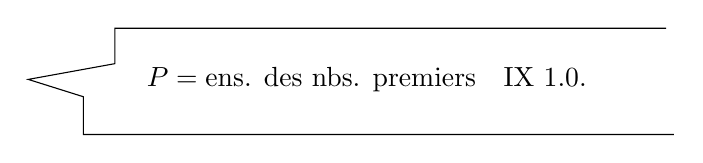
\begin{tikzpicture}
\node[align=left] at (0,0) {\handwritten{$\mathbb{P}={}$ens. des nbs. premiers\quad IX 1.0.}};
\draw (3.8,.65)--(-3.2,.65)--(-3.2,.2)--(-4.3,0)--(-3.6,-.22)--(-3.6,-.7)--(3.9,-.7);
\end{tikzpicture}}

faisceau de ind-p-groupes, faisceau de groupes ind-finis\quad sheaf of ind-p-groups, sheaf of ind-finite groups\quad \unsure{IX|YX} 1.5

localement constant (faisceau - )\quad locally constant sheaf\quad IX 2.0

constructible (faisceau d'ensembles, de groupes, de modules - )\quad constructible \deleted{\unsure{(}} sheaf of sets, groups or modules\deleted{)}\quad IX 2.3

connexe par arcs (schéma - )\quad arcwise connected scheme\quad IX 2.12

Kummer (théorie de - )\quad IX 3.2

\figure{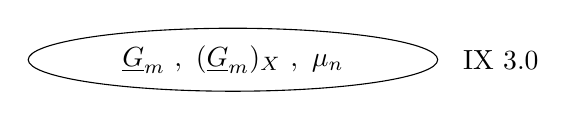
\begin{tikzpicture}
\node at (0,0) {$\underline{G}_m\ ,\ (\underline{G}_m)_X\ ,\ \handwritten{\mathbb{\mu}}_n$};
\draw (0,0) ellipse (2.6cm and .4cm);
\node[anchor=west] at (2.8,0) {IX 3.0};
\end{tikzpicture}}

Hilbert (théorème 90 de - )\quad IX 3.3

diviseur de Cartier\quad Cartier divisor\quad IX 3.4

Artin-Schreier (théorie de - )\quad IX 3.5

\figure{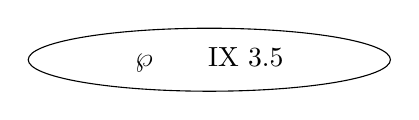
\begin{tikzpicture}
\node at (0,0) {$\handwritten{\wp}$\qquad IX 3.5};
\draw (0,0) ellipse (2.3cm and .4cm);
\end{tikzpicture}}

fa\deleted{\unsure{s}}i\deleted{\unsure{i}}sceau gratte-ciel\quad skyscraper sheaf\quad IX 4.1

morphisme trace\quad trace morphism\quad VIII 5.1 , XVII ...
\margin{\handwritten{*}}

$\handwritten{\ell}$-dimension cohomologique \inserted{d'un schéma}\quad $\handwritten{\ell}$-cohomological dimension \inserted{of a scheme}\quad X 1
\margin{\handwritten{$\ell$}}

\figure{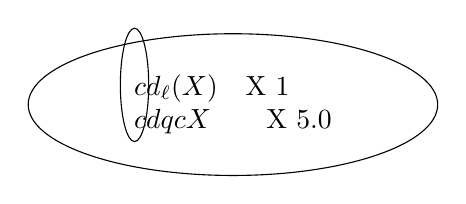
\begin{tikzpicture}
\node[align=left] at (0,0) {$\operatorname{cd}_{\handwritten{\ell}}(X)$\quad X 1\\$\operatorname{cdqc}X$\qquad X 5.0};
\draw (0,0) ellipse (2.6cm and .9cm);
\draw (-1.25,.25) ellipse (.18cm and .72cm);
\end{tikzpicture}}
\margin{\handwritten{$\ell$}}

fibration élémentaire\quad elementary fibration\quad XI 3.1

bon voisin\deleted{\unsure{g}}age (relativement à $S$)\quad nice neighbour\deleted{\unsure{h}}hood relative to $S$\quad \inserted{XI 3.2}

théorème de comparaison\quad comparison theorem\quad XI 4.4

\figure{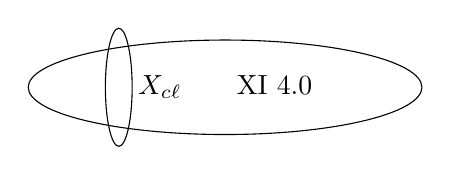
\begin{tikzpicture}
\node at (0,0) {$X_{c\handwritten{\ell}}$\qquad XI 4.0};
\draw (0,0) ellipse (2.5cm and .6cm);
\draw (-1.35,0) ellipse (.17cm and .75cm);
\end{tikzpicture}}

\figure{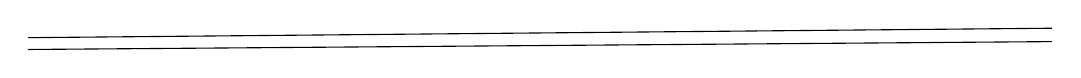
\begin{tikzpicture}\draw (0,0)--(13,.12);\draw (0,-.15)--(13,-.05);\end{tikzpicture}}
\margin{\handwritten{\uline{Vol. 2}}}

théorème de changement de base propre\quad proper base change theorem\quad XII 5.1

morphisme de changement de base\quad base change morphism\quad XII 4 , XVIII ...
\margin{\handwritten{*}}
% archive sheet number: 42
